\documentclass{article}
\usepackage[utf8]{inputenc}
\usepackage{mathtools}
\usepackage{pgfplots}
\usepackage{natbib}
\usepackage{amsmath}
\usepackage{amssymb}
\usepackage{amsfonts}
\usepackage{natbib}
\usepackage{graphicx}
\usepackage{minted}
\usepackage{ dsfont }
\usepackage{xcolor}
\usepackage{adjustbox}
\usepackage{soul}


\usepackage[a4paper,margin=1in,footskip=0.25in]{geometry}
\allowdisplaybreaks


\title{CSE546 Machine Learning HW4}
\author{Bobby Deng | 1663039 | dengy7 }
\date{1 June 2020}

\begin{document}
\maketitle

\section*{A1. Conceptual Questions}
\subsection*{a.}
Yes, this is true. GD converges to global min when the local min happens to be the global min.


\subsection*{b.}
False, it is not a good practice to make weights initiated as 0. For example, if we use Sigmoid activation function, the gradient is always zero no matter how many iteration passed. And basically setting weights to zero is not better than a simple linear model.

\subsection*{c.}
False, we use none-linear function to enable back propagation for multiple layers. The linear activation function will produce a linear transformation for the input.

\subsection*{d.}
False, they both can be solved by using matrix multiplication. Only thing is that back propagation used more GPU memory. I relies on the output of the forward pass which has to be cached for backward pass use which resulting using a lot of GPU memory. 


\subsection*{e.}
False, this depends on the different situations. In some case PCA gets smaller reconstruction error, and in some cases AE has lower reconstruction error. PCA is restricted to a linear map, however AE allow none-linear encoder and decoders.

\section*{A2. }

\subsection*{a.}
1. Problems when police respond differently in different neighborhoods.
For example, police might distribute more resources in rich communities and less resource in poor communities. And we know that usually poor communities will have more crimes than rich communities. And this will lead to a disproportionate distribution of resources and may lead to more crime in poor community and wasted resources in rich communities. \\

2. 

\subsection*{b.}





\subsection*{c.}



\section*{A4. }

\subsection*{a.}
This part of question, I used pre-trained AlexNet and only modify the last output layer since we only have 10 classes on CIFAR-10. \\
Best Training Accu:  0.740925 \\
Best Validation: 0.7346 \\
Test Accu:  0.7396 \\

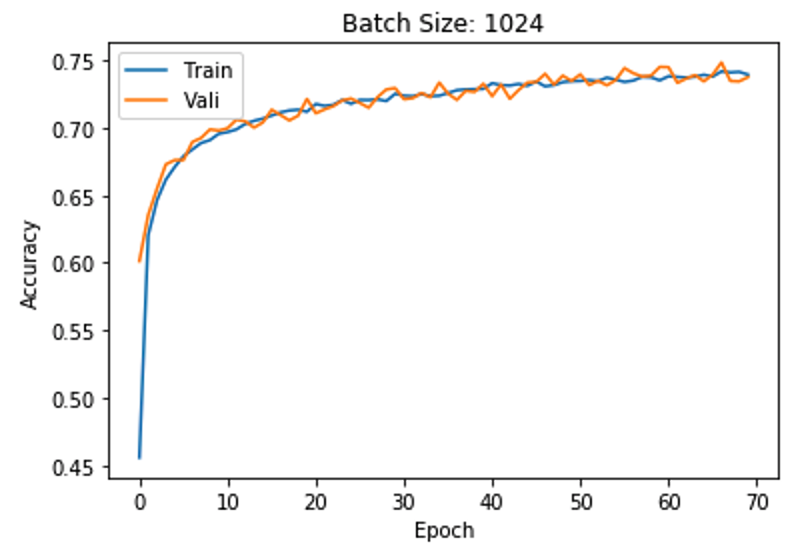
\includegraphics[width=9cm, height=6cm]{plots/A4a.png}


\subsection*{b.}
In this question, we use AlexNet but we randomize all parameters in the net to start with. \\
Best Training Accu:  0.873625 \\
Best Validation Accu:  0.8702 \\
Test Accu: 0.86944 \\

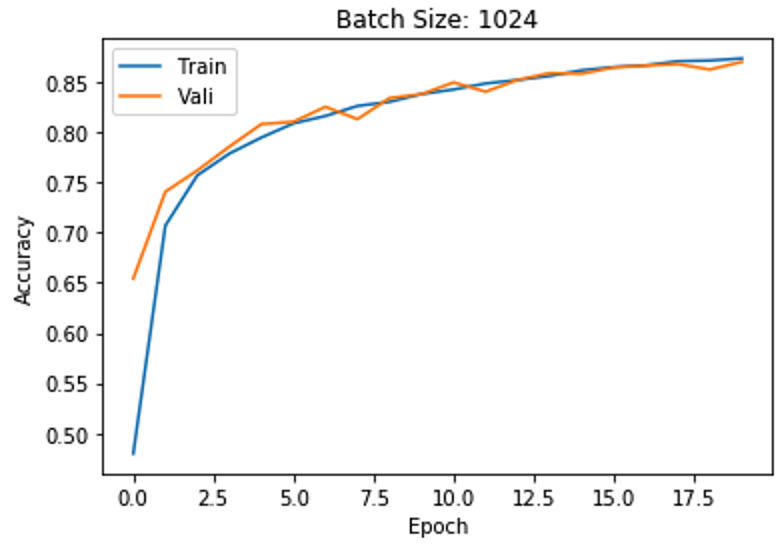
\includegraphics[width=9cm, height=6cm]{plots/A4b.png}


\section*{A5. }

\subsection*{a.}
Best vali accu: 0.2874 \\
Best test accu: 0.2754 \\
Best param set: {'lr': 0.005, 'momentum': 0.9} \\

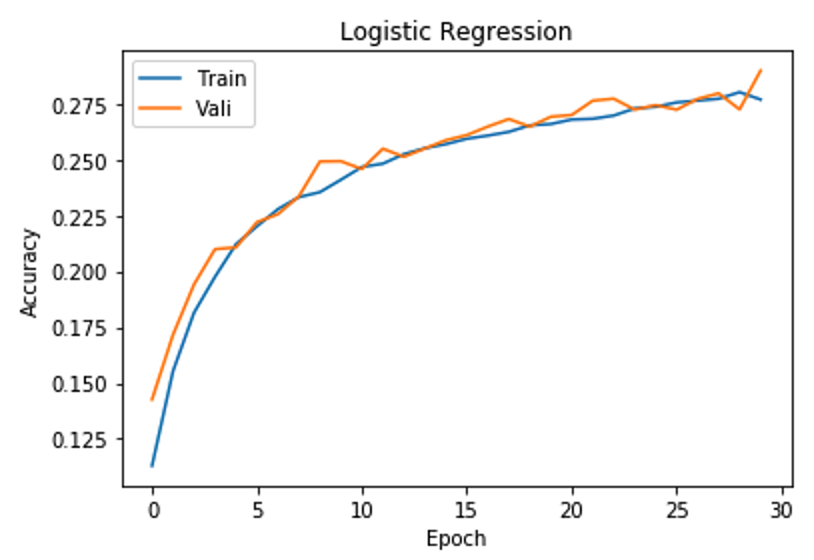
\includegraphics[width=7cm, height=6cm]{plots/A5a_0.png}
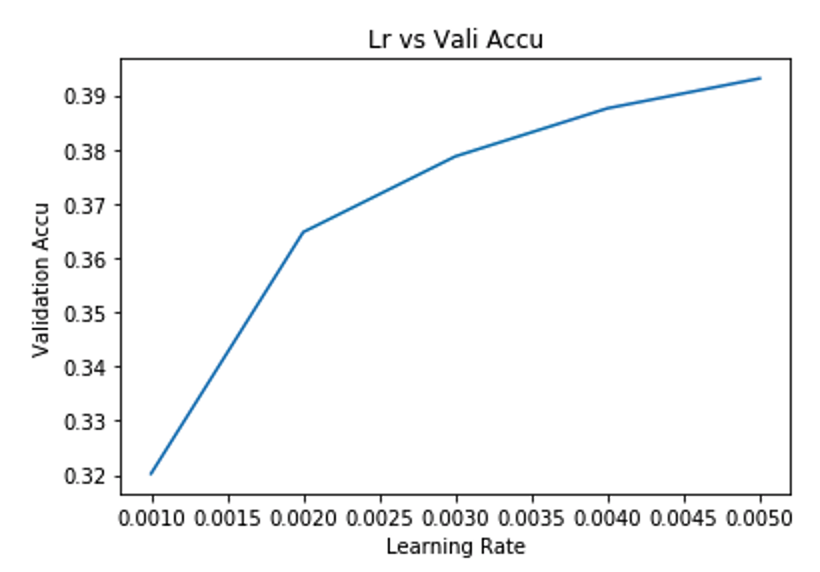
\includegraphics[width=7cm, height=6cm]{plots/A5a_1.png} \\
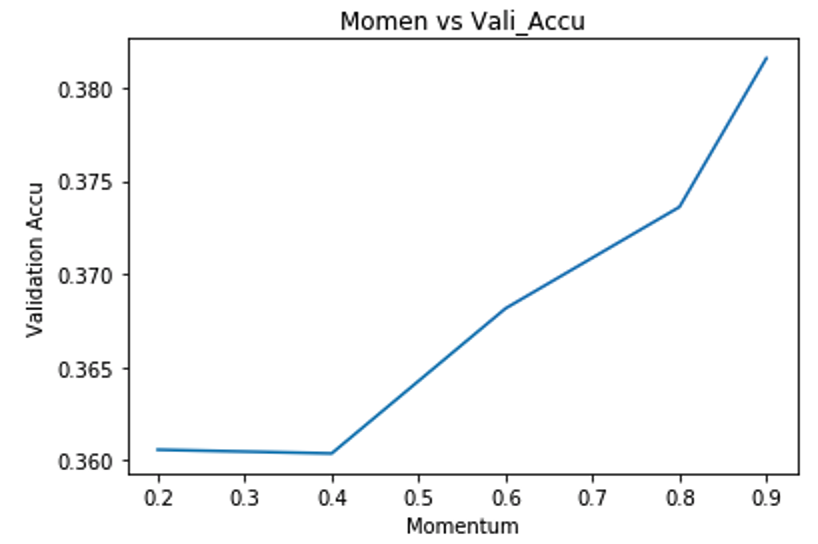
\includegraphics[width=7cm, height=6cm]{plots/A5a_2.png}

\subsection*{b.}
Best vali accu: 0.3902 \\
Best test accu: 0.3921 \\
Best param set: {'lr': 0.005, 'momentum': 0.9, 'M': 150} \\
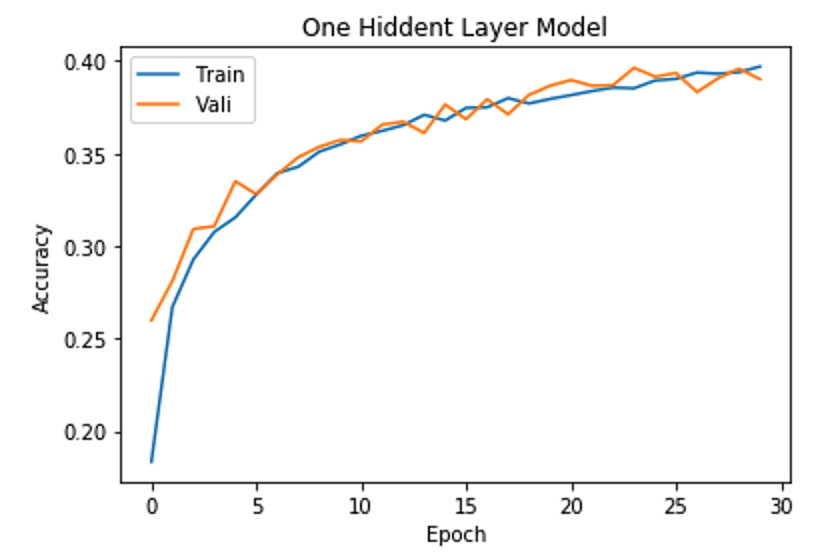
\includegraphics[width=7cm, height=6cm]{plots/A5b.png} 
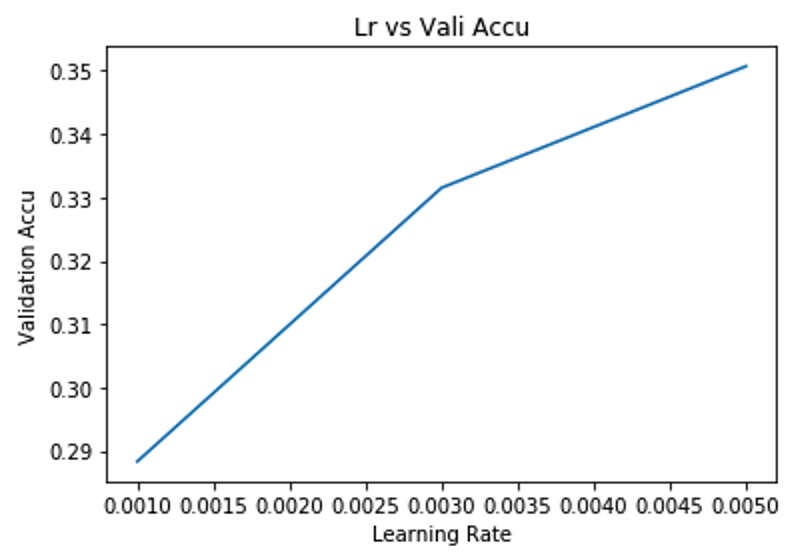
\includegraphics[width=7cm, height=6cm]{plots/A5b_1.png} \\
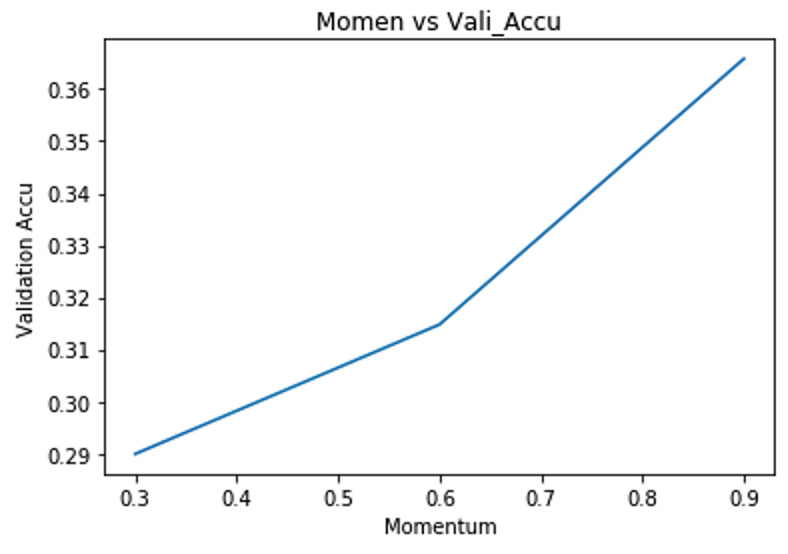
\includegraphics[width=7cm, height=6cm]{plots/A5b_2.png}
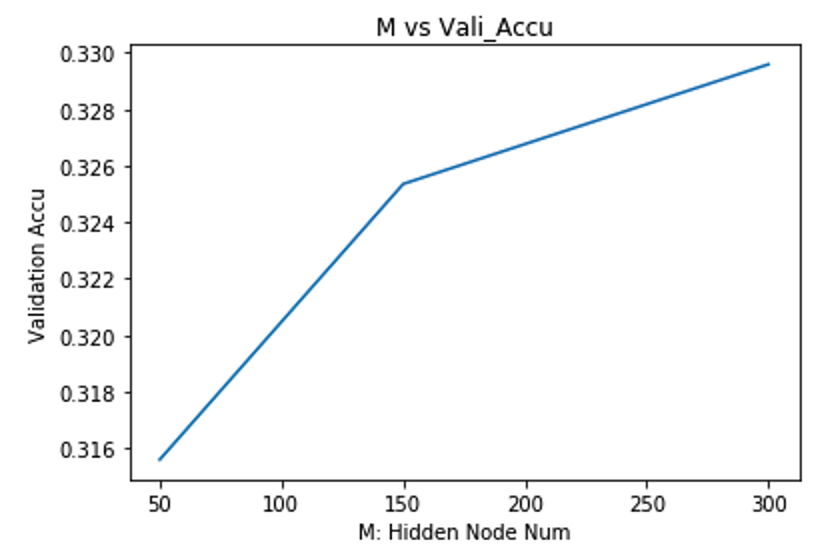
\includegraphics[width=7cm, height=6cm]{plots/A5b_3.png} \\

\subsection*{c.}


\subsection*{d.}
Test Accu: 0.7094, 423 epochs \\
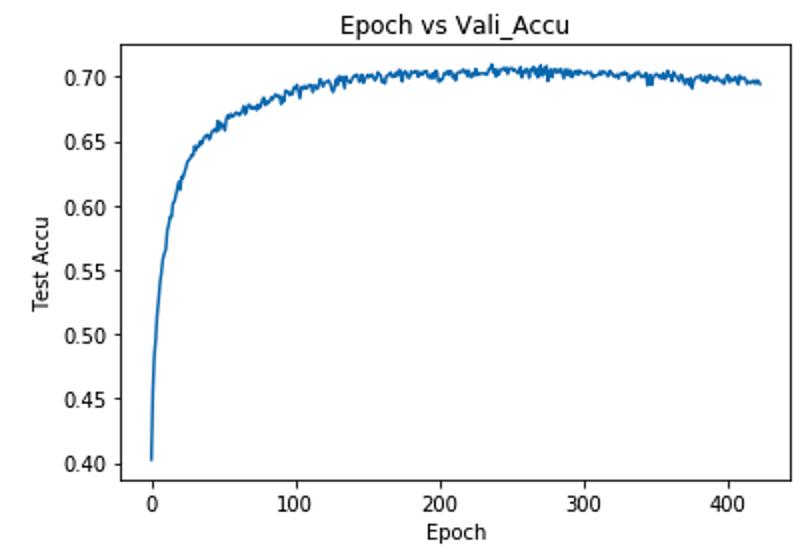
\includegraphics[width=7cm, height=6cm]{plots/A5d.png}
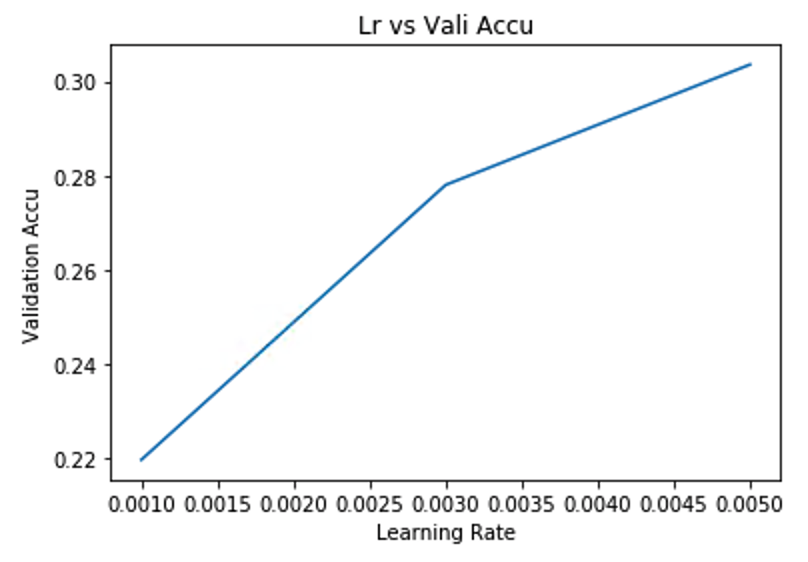
\includegraphics[width=7cm, height=6cm]{plots/A5d_1.png} \\
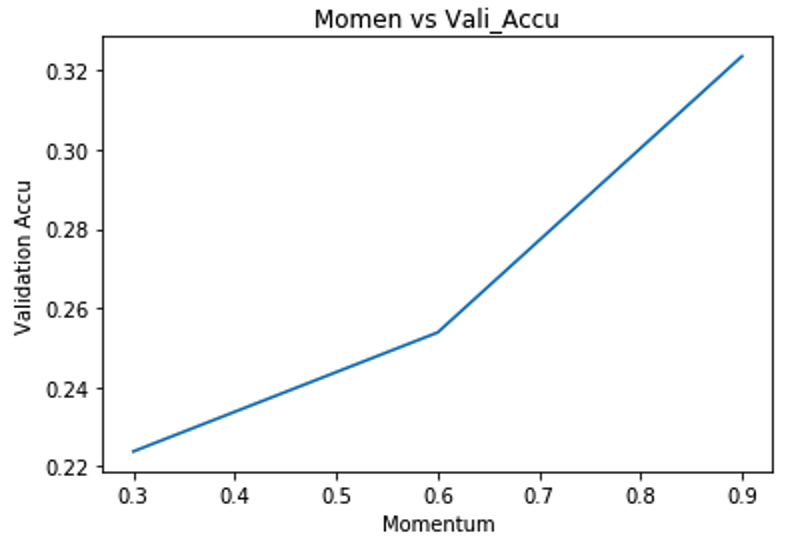
\includegraphics[width=7cm, height=6cm]{plots/A5d_2.png}
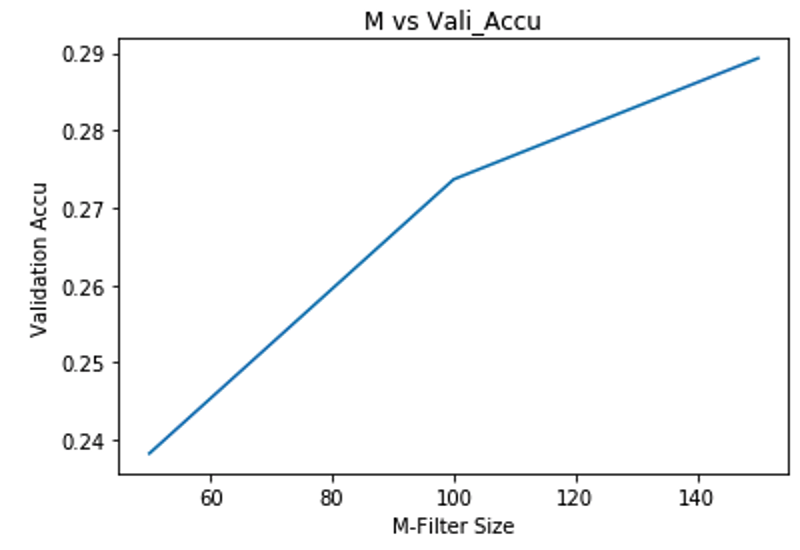
\includegraphics[width=7cm, height=6cm]{plots/A5d_3.png} \\

\end{document}